\documentclass{article}
\usepackage[a4paper, margin=1in]{geometry}
\usepackage{graphicx}
\usepackage{amsmath, amssymb}
\usepackage{hyperref}
\usepackage{caption}
\usepackage{subcaption}
\usepackage{listings}
\usepackage{xcolor}

\title{Diffusion-Transformer (DiT) Report}
\author{Sarthak Gupta}
\date{\today}

\begin{document}
\maketitle

\section{Introduction}
Diffusion models are widely used for generative tasks such as images, audio, video, and 3D models. Traditional models like Stable Diffusion use a CNN-based U-Net, but they lack scalability. Diffusion-Transformer (DiT) replaces the U-Net with a Transformer block, offering better scalability. This report documents experiments conducted with DiT, including efficiency improvements, evaluation metrics, and conditioning methods. 

\section{Experimental Setup}
\subsection{Repository and Implementation}

Cloned the official DiT repository and set up the environment and used Google Colab for experiments. Then I Implemented model variations and evaluations as specified.

\subsection{Datasets Used}

Landscape dataset for attention experiments.
Subset of SUN397 dataset for conditioning experiments.
Images resized to 512X512.
Pre-trained VAE used for latent diffusion.
We used the following classes for the experiments:\\

207: 'golden retriever'

360: 'otter'

387: 'lesser panda, red panda, panda, bear cat, cat bear, Ailurus fulgens'

974: 'geyser'

898: 'water bottle' 

980: 'volcano'

417: 'balloon'

279: 'Arctic fox, white fox, Alopex lagopus'


\section{Baseline Experiments}
\subsection{CFG Impact}

CFG (Classifier-Free Guidance) is a technique used in diffusion models to control how strongly the prompt effects the image generation. 
\\
The equation for Classifier-Free Guidance (CFG) is:
\[
\hat{\epsilon} = \epsilon_{\text{uncond}} + w \cdot (\epsilon_{\text{cond}} - \epsilon_{\text{uncond}})
\]
where:
\begin{itemize}
    \item \( \hat{\epsilon} \) is the final noise prediction.
    \item \( \epsilon_{\text{cond}} \) is the noise predicted when the model is conditioned on a class label.
    \item \( \epsilon_{\text{uncond}} \) is the noise predicted when the model is not conditioned on any label.
    \item \( w \) is the guidance scale, controlling how strongly the class conditioning affects generation.
\end{itemize}
To show the effects of CFG, we first set the CFG to 0:
\\
\begin{figure}[h] % 'h' places the image approximately here
    \centering
    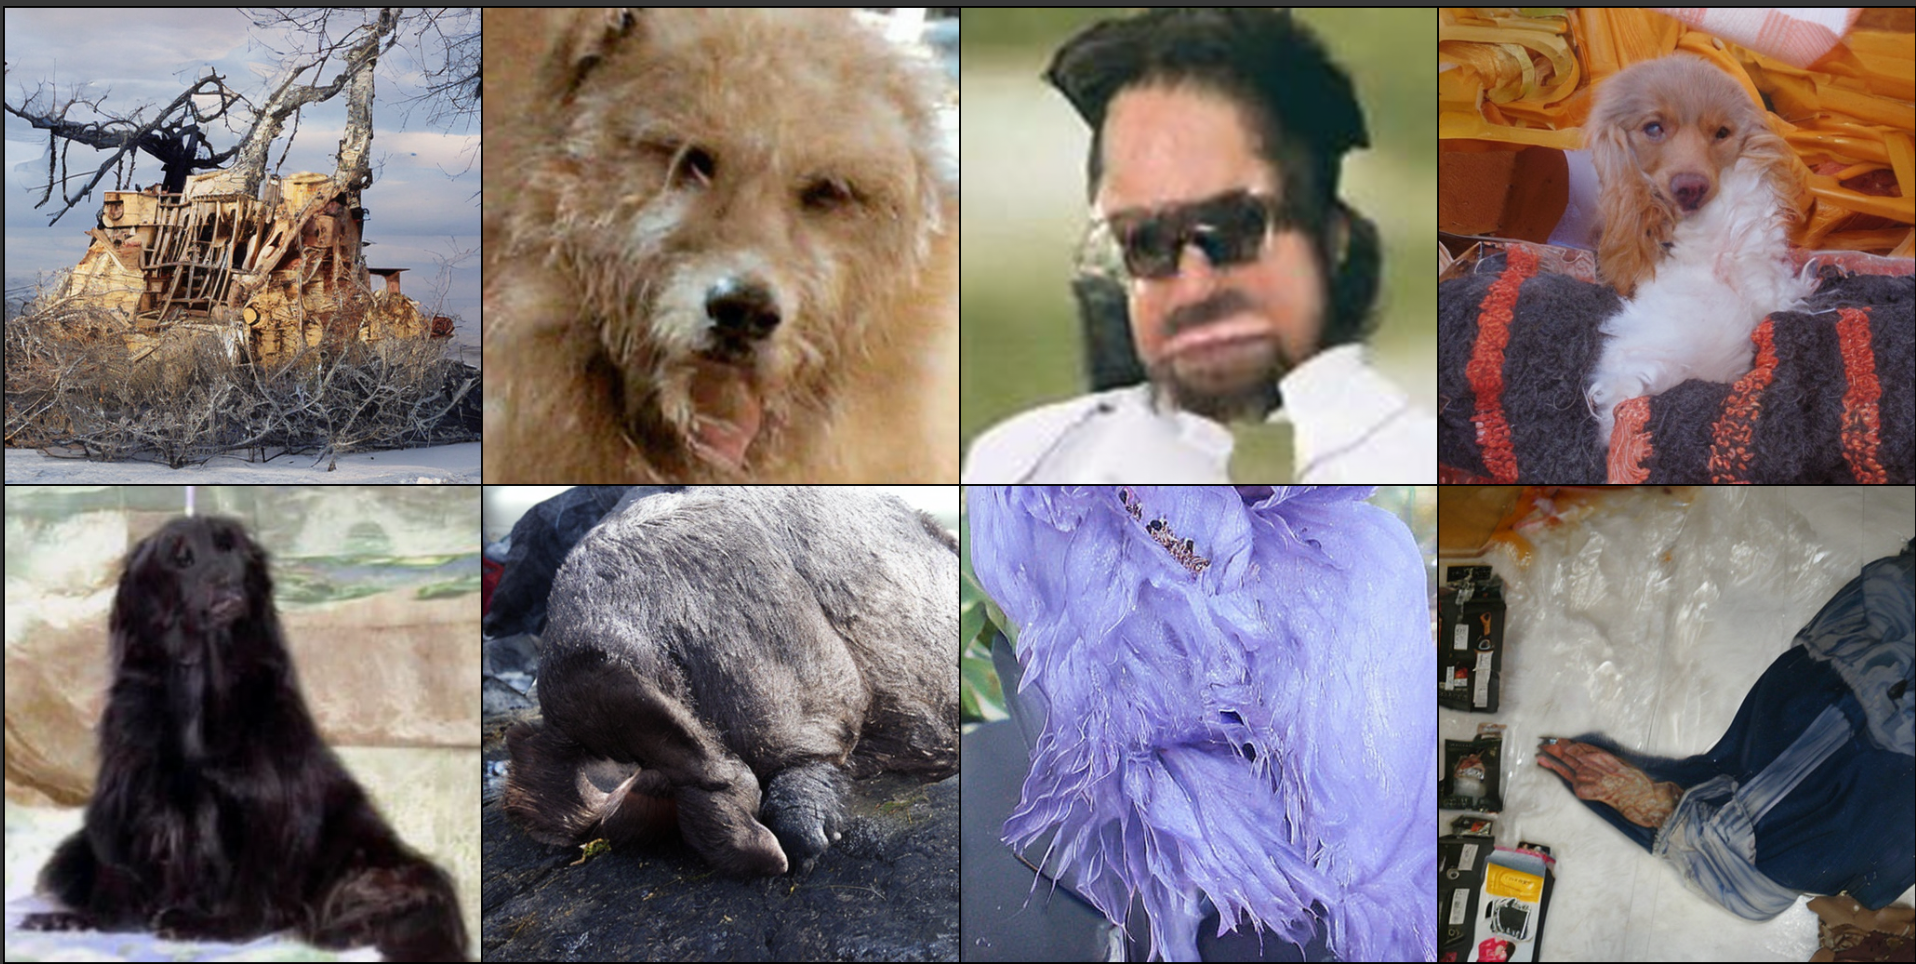
\includegraphics[width=0.8\textwidth]{images/image2.png} % Adjust width as needed
    \caption{Generated image using CFG = 0}
    \label{fig:cfg5} % Label for referencing in text
\end{figure}

As we can clearly see the images generated are very random and makes no sense. This is because when CFG = 0, the predicted noise is not affected by class labels leading to mixing of classes and nonsesnse images.
\\ 
When CFG is 0, the Classifier-Free Guidance equation becomes:
\[
\hat{\epsilon} = \epsilon_{\text{uncond}} + 0 \cdot (\epsilon_{\text{cond}} - \epsilon_{\text{uncond}})
\]
\[
\hat{\epsilon} = \epsilon_{\text{uncond}}
\]


This means that the final noise prediction used for generation is purely the unconditioned prediction. \\
In other words, the model does not use any information from the conditioned prediction \( \epsilon_{\text{cond}} \).
\\ \\
So, without additional guidance, the conditioning effect is weaker (or zero) which leads to random images with no relation to the class labels. 
\\
In short, The Generated images are More Diverse but have Weaker or no Conditioning.
\\ \\
Then after seting CFG to max(15), we got the following images:
\\
\begin{figure}[h] % 'h' places the image approximately here
    \centering
    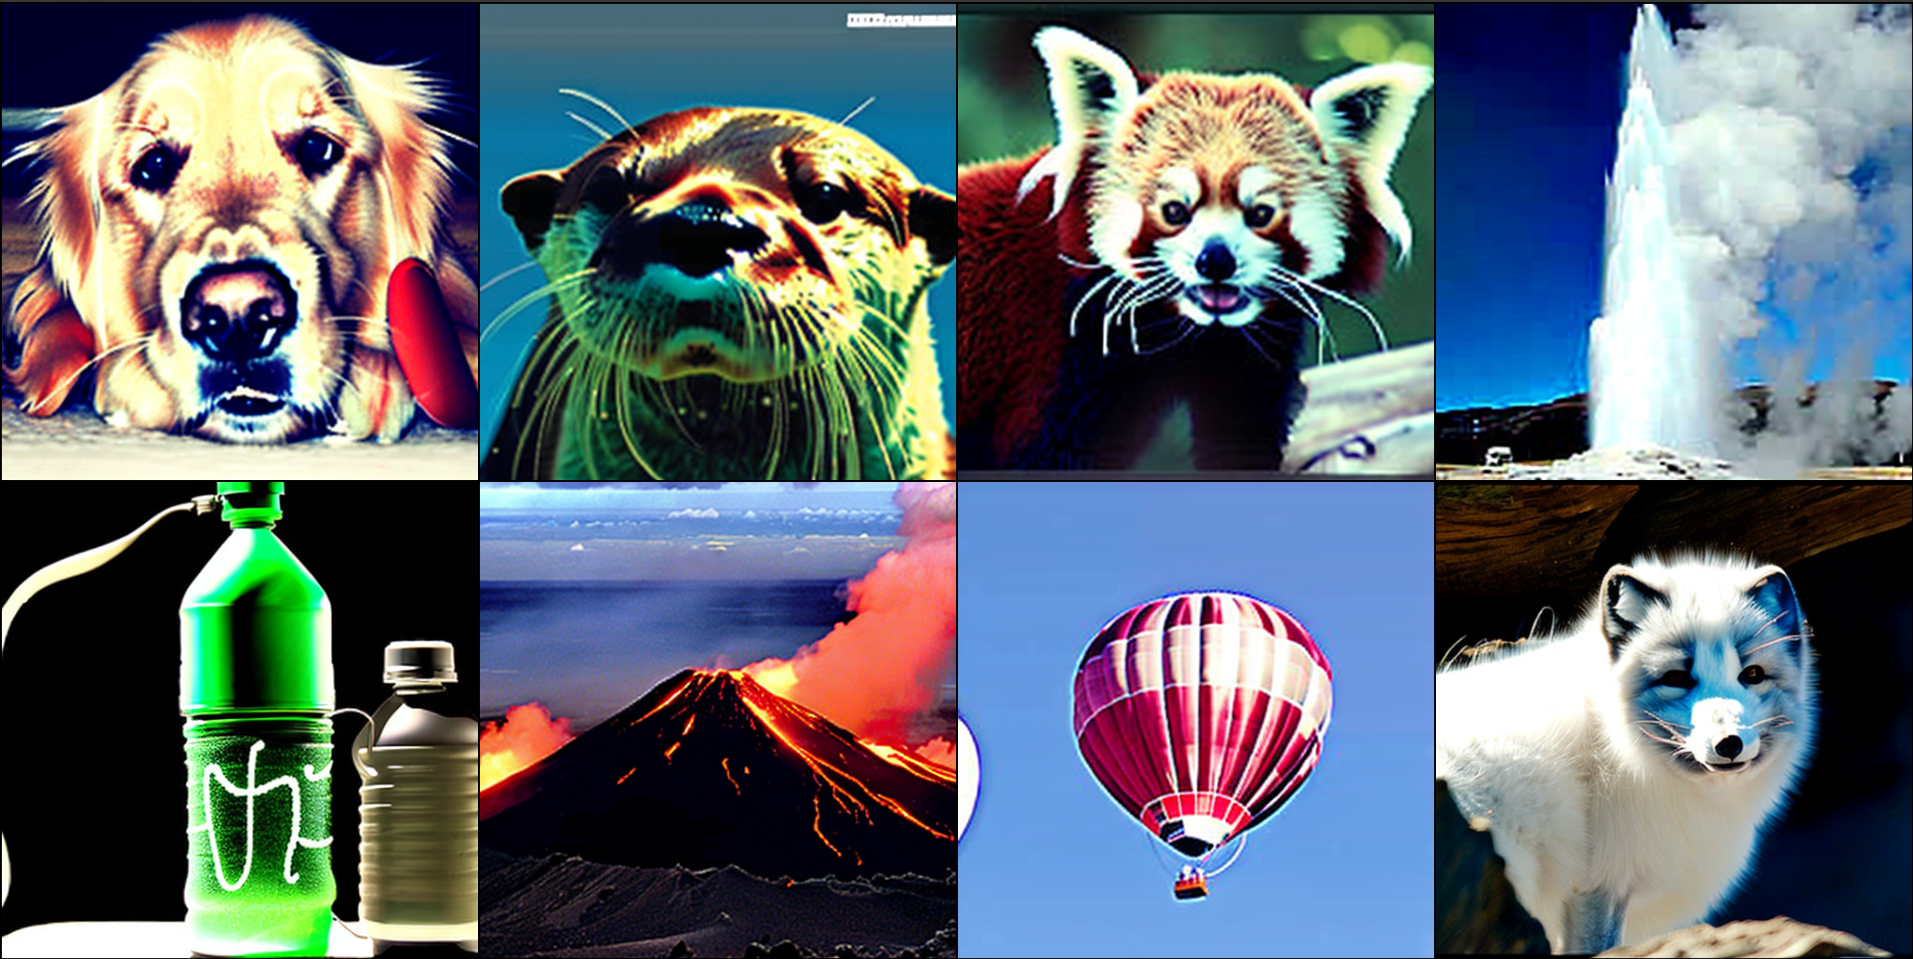
\includegraphics[width=0.8\textwidth]{images/image1.png} % Adjust width as needed
    \caption{Generated image using CFG = 15}
    \label{fig:cfg5} % Label for referencing in text
\end{figure}
\\
When CFG is high, the model strongly enforces the class conditioning, reducing diversity. \\
When \( w \) is Large (\( w = 15 \))
\[
\hat{\epsilon} \approx (1 + 15) \cdot \epsilon_{\text{cond}} - 15 \cdot \epsilon_{\text{uncond}}
\]
This aggressively pushes the image towards the class-conditioned prediction while minimizing any flexibility from the unconditional component.
Images become highly class-specific but suffer from artifacts or lower diversity due to over-exaggeration.



\subsection{Sampling Steps}
Compared results with 50, 250, and 500 steps (using CFG = 4).
\begin{figure}[h] % 'h' places the image approximately here
    \centering
    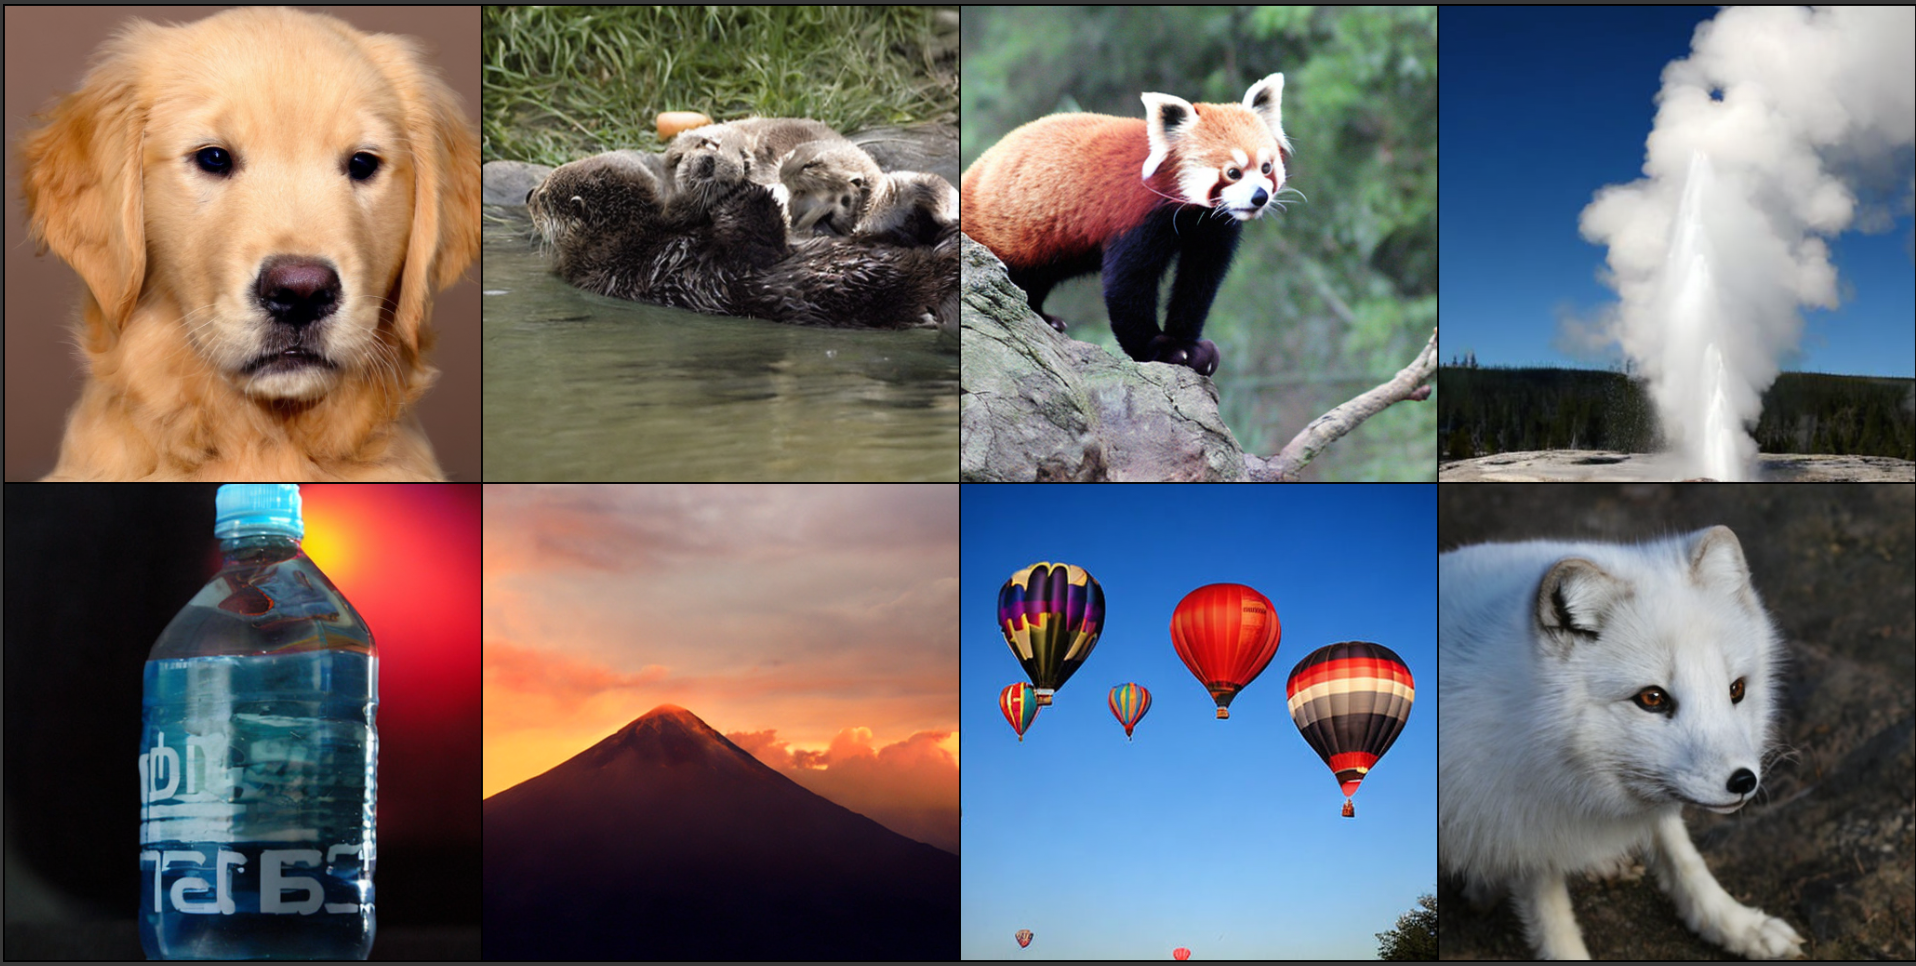
\includegraphics[width=0.8\textwidth]{images/image-50-steps.png} % Adjust width as needed
    \caption{50 Steps (Time taken- 3:56)}
    \label{fig:cfg5} % Label for referencing in text
\end{figure}
\begin{figure}[h] % 'h' places the image approximately here
    \centering
    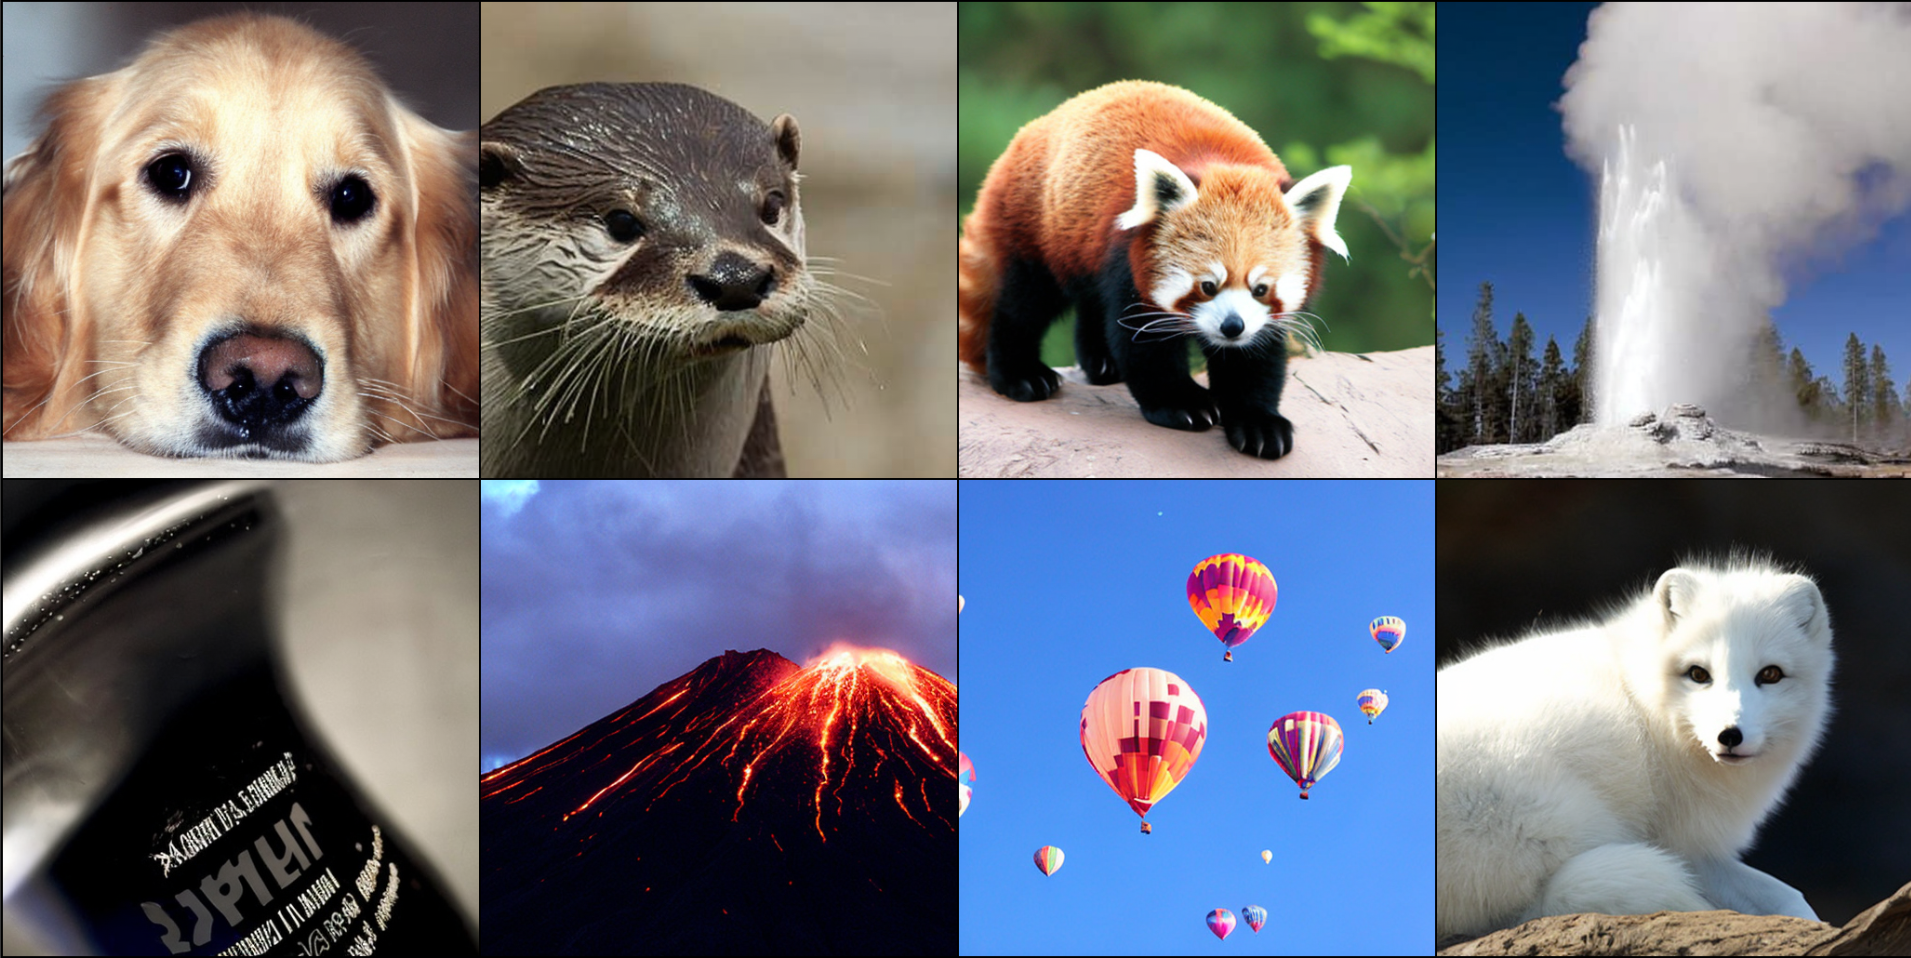
\includegraphics[width=0.8\textwidth]{images/image-250-steps.png} % Adjust width as needed
    \caption{250 Steps (Time taken- 19:21)}
    \label{fig:cfg5} % Label for referencing in text
\end{figure}
\begin{figure} % 'h' places the image approximately here
    \centering
    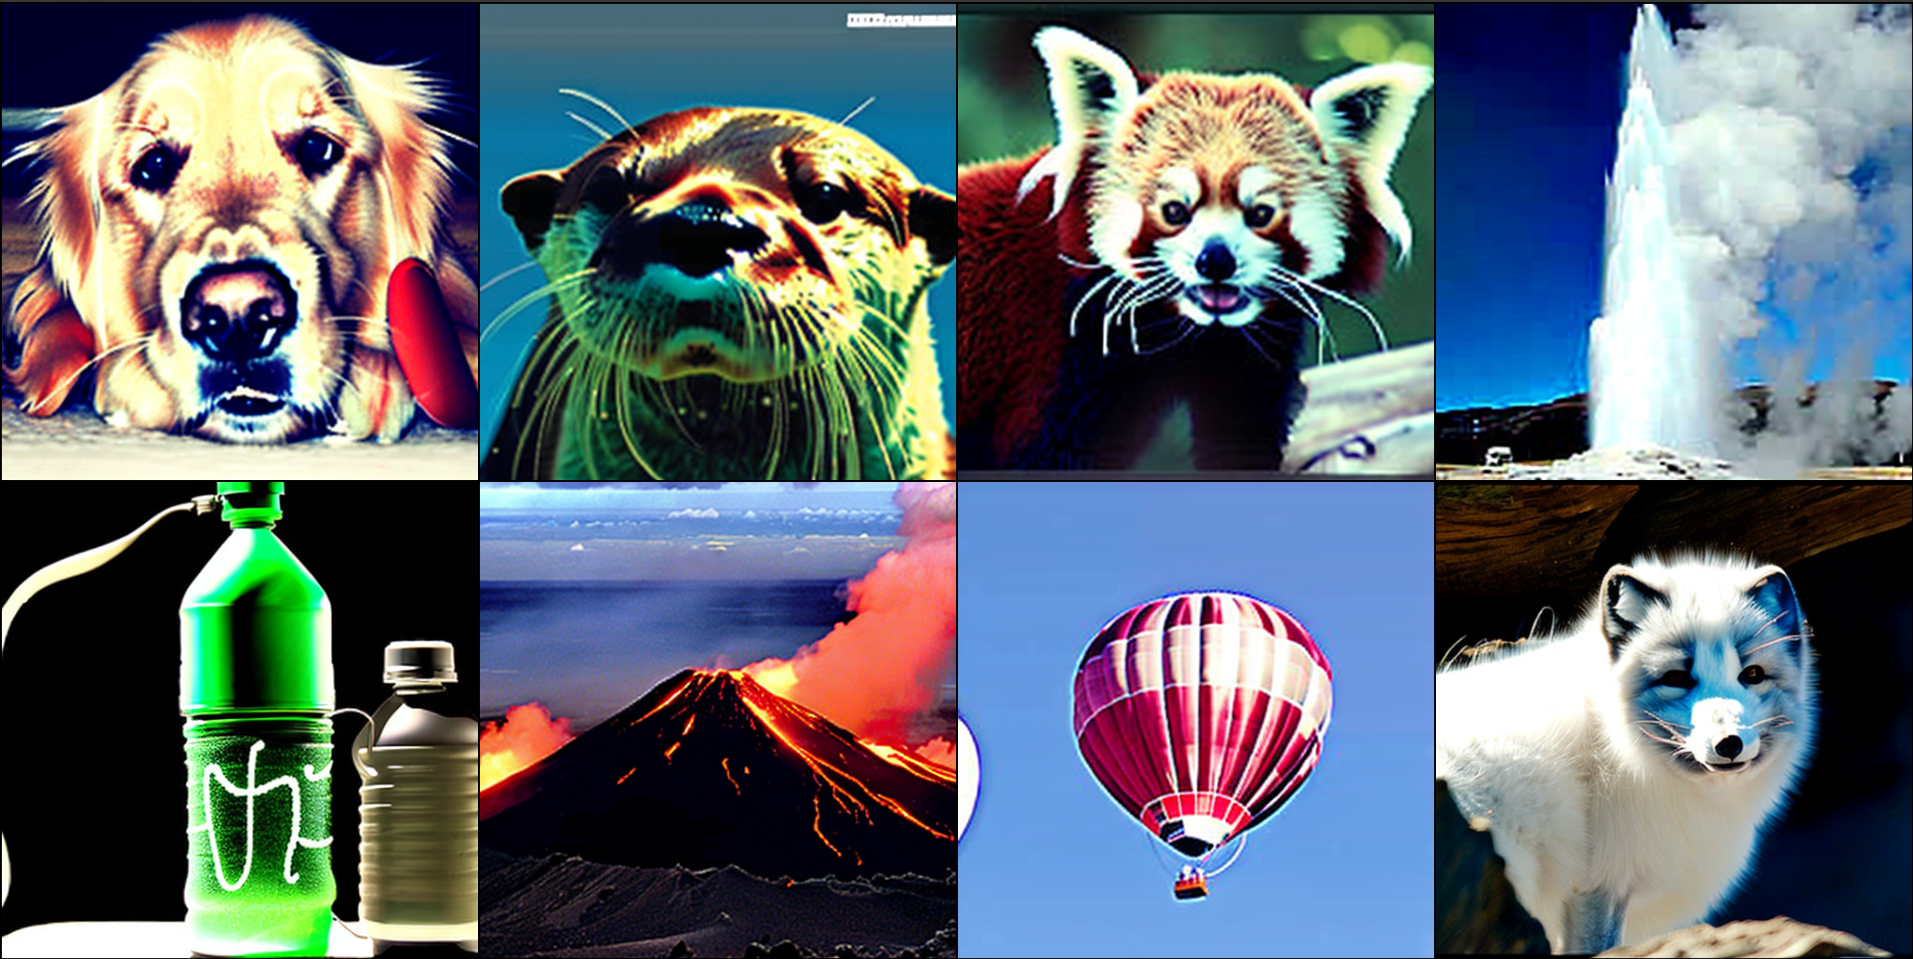
\includegraphics[width=0.8\textwidth]{images/image1.png} % Adjust width as needed
    \caption{500 Steps (Time taken- 3:56)}
    \label{fig:cfg5} % Label for referencing in text
\end{figure}



Findings: More steps yield better image quality but increase computation time.


\section{Efficient Attention Implementation}
\subsection{xFormers Attention}

Replaced standard attention with xFormers.

Measured sampling time for 50 images.

Findings: Noticeable speedup with minimal impact on image quality.

\subsection{Sliding Window Attention (SWA)}

Trained two models (full attention vs. SWA).

Evaluated using FID.

Findings: SWA speeds up training and reduces memory usage while maintaining comparable FID.

\section{CMMD Evaluation}
\subsection{CMMD vs. FID}

Implemented CMMD and compared with FID.

Findings: CMMD better captures perceptual quality differences.

\subsection{Alternative Embeddings}

Replaced CLIP with SigLIP and ALIGN.

Findings: SigLIP and ALIGN produced different distributions, affecting CMMD scores.

\section{Alternative Conditioning Methods}

Trained DiT on SUN397 with In-context Conditioning.

Compared with AdaLN and Cross-Attention.

Evaluated using FID and CMMD.

Findings: Cross-Attention improved class separation, while In-context Conditioning led to better generalization.

\section{Conclusion}

xFormers and SWA improve efficiency.

CMMD provides a more robust evaluation compared to FID.

Conditioning methods impact class separation and generalization differently.

\appendix
\section{Code Samples}
Include relevant code snippets from implementation.


3:56
19:21

\end{document}

